\comment{
\begin{figure}
(a) DDMS: show state machine, with databases as states and updates as transitions.

(b) DBMS: database sits and waits for queries to arrive; answers them.

(c) Data stream processor: Set of sitting queries; a stream of data passes by.

\caption{Data management systems architectures: DDMS vs. DBMS vs. data stream processors.}
\end{figure}
}

\begin{figure}
\begin{center}
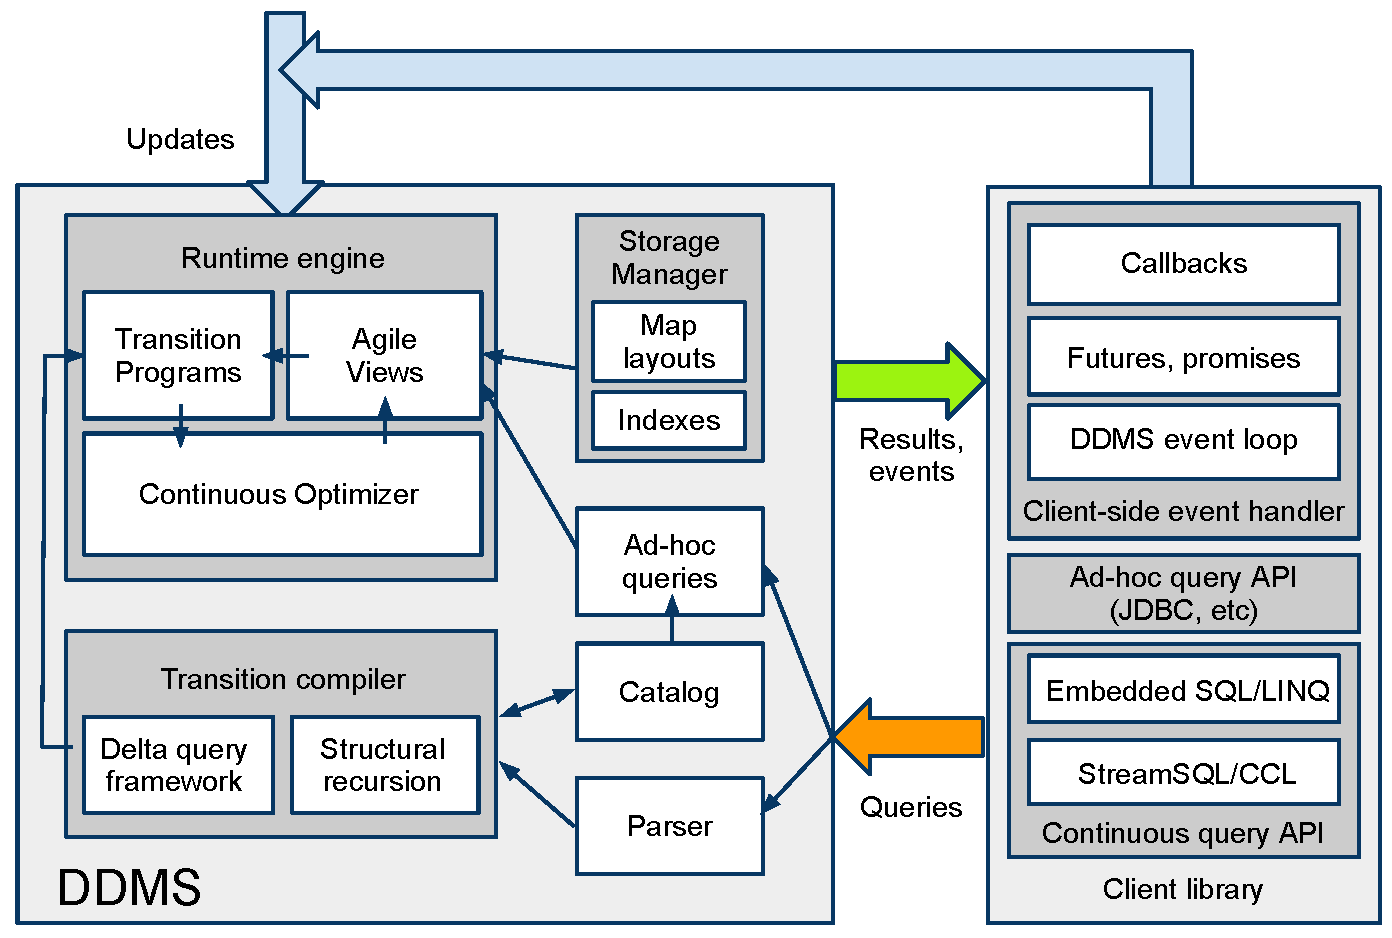
\includegraphics[width=3.3in]{graphics/CIDRarch.pdf}
\end{center}
\vspace*{-0.2in}
\caption{Dynamic Data Management System (DDMS) and Application Interface
Architecture}
\label{fig:ddmsarch}
\vspace*{-0.2in}
\end{figure}

We now examine the architecture of a DDMS, as illustrated in Figure \ref{fig:ddmsarch}.  The core component of a DDMS is its runtime engine.  Unlike a traditional database system where the same runtime code manages all database instances, each instance of a DDMS execution runtime is constructed around a specific set of queries provided by the client program (eg., via SQL code embedded inline in the program), each of which defines an \textit{agile view}.

An important distinction between the DDMS and a traditional DBMS, is that the DDMS treats both its inputs (base relations in DBMS parlance) and agile views (query outputs) as \textit{update streams} of tuple insertions, deletions and revisions.  Updates are processed, and changes in the agile views are propagated into the client.  If necessary, a DDMS runtime can also be instantiated with support for ad-hoc queries, but the DDMS treats this as a secondary concern.

The client-provided agile views, or \textit{visible schema} form the primary read interface between client programs and a DDMS runtime.  This interface comes in three flavors: (1) a push interface that invokes client callbacks or schedules event handlers when the value of the visible schema changes, (2) futures/promises representing queries over the visible schema that have not yet been computed, or (3) read-only \textit{dynamic datastructures} representing each view in the \textit{visible schema}.  As an aside, an interesting consequence of limiting visibility into the database to the visible schema is that we are free to represent a DDMS runtime's internal state in ways that are dramatically different from a traditional DBMS.  We return to this observation later in the paper.

{\bf The runtime state machine}\/.
The internals of the runtime engine itself are best viewed through the lens of a state machine.  Compared to similar abstractions for stream processors\cite{demers-sigmod:07}, the state is substantially larger; conceptually at least, the state represents an entire relational database.  In this model, transitions represent changes in the base relations: events in the update stream.

{\bf Compiling transitions}\/.
Each transition is effectively a query for each view of interest.  Though the subqueries are simpler, it is not enough to make a DBMS-style query workload tenable in a high-performance system.  However, instead of reevaluating the subquery on every transition, we can the subquery as simply another agile view.  These views - the \textit{auxiliary schema} - are generated by a compilation process discussed further in Section \ref{sec:dbtoaster}.  

{\bf Space vs speed, partitioning and other optimizations}\/.
The entire \textit{relevant} state of the database is completely expressed through the auxiliary and visible schemas.  However, substantial room exists for optimization tradeoffs.  For example, the compiler may choose to compute one or more views on the fly, rather than maintaining it in order to keep expected space usage within predefined bounds.  At runtime, the engine invokes a continuous query optimizer that guides the decisions to be made across the database schema, state and storage.  The optimizer's decisions are made in terms of the space being used, the cost of applying transitions on updates, as well as information from a storage manager that aids in physical aspects of handling large states, including implementing a variety of layouts and indexes to facilitate processing.
